
\documentclass[8pt]{article}
%	options include 12pt or 11pt or 10pt
%	classes include article, report, book, letter, thesis

\usepackage[a4paper,bindingoffset=0.2in,%
            left=0.6in,right=0.6in,top=0.2in,bottom=0.4in,%
            footskip=.15in]{geometry}
            
\usepackage[T1]{fontenc}
\usepackage[polish]{babel}
\usepackage[utf8]{inputenc}
\usepackage{lmodern}
\selectlanguage{polish}
\usepackage{blindtext}
\usepackage{pgfplots}
\usepackage{graphicx}


\title{Algorytmy numeryczne}
\author{Zadanie 2 \\ Aleksander Kosma | Tomasz Adamczyk\\grupa 1 tester-programista}
\date{8 Listopad 2017}

\begin{document}
\maketitle 

\section{Dodawanie i Mnożenie}

Opracowanie prezentuje obliczenia na macierzach, przy użyciu języka java i wsparciu biblioteki eigen 
wykorzystanego w C++.
Pierwsza część opisuje czas działania i błędy operacji dodawania i mnożenia.
Obliczenia wygenerowane w javie porównywane były z wynikami wygenerowanymi z eigena.
Testy zostały przeprowadzone na 3 wzorach:
$$A * X\qquad \qquad \qquad  (A+B+C)*X \qquad \qquad \qquad A*B*C$$
Gdzie litery A,B,C to macierze, X to wektor.
Testy zostały przeprowadzone na 3 typach zmiennych. Double, Float i na własnym typie, który przechowuje
liczbę w postaci ułamka. Typ ten ma bezstratną precyzję. Liczby które rozstały
wykorzystane do obliczeń mieściły się w przedziale od 0 do 1, w postaci dziesiętnej, z wykorzystaniem precyzji double.

Pierwsze dwa wykresy prezentują czas potrzebny do obliczenia podanego wzoru. Oś pionowa reprezentuje czas w sekundach,
oś pozioma rozmiar macierzy. Podane wykresy utworzone zostały  na zmiennej double.\\
\begin{center}
 \makebox[\textwidth]{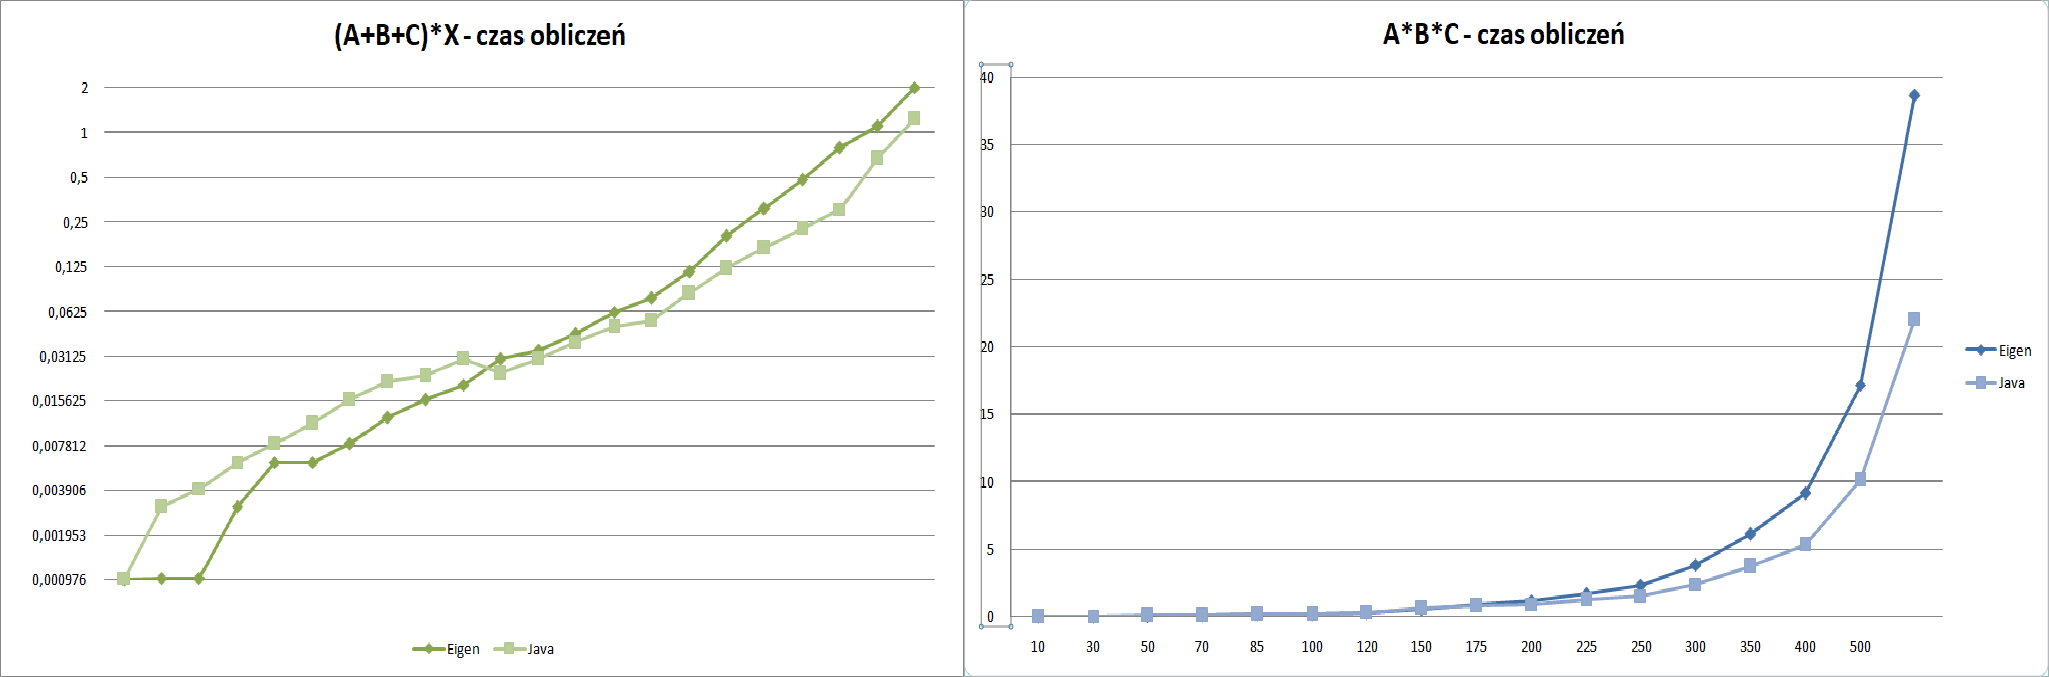
\includegraphics[width=20cm,height=7cm]{CzasRazem.png}}
\end{center}



Kolejne dwa wykresy odnotowują uzyskana precyzje. Wyznaczona ona była poprzez wyznaczenie średniej wartości
dla końcowej macierzy i odjecie od siebie wyniku z eigena i javy. Widać ze wraz ze wzrostem wielkości macierzy,
błędy przybierają na wartości.Tym większa macierz tym większy błąd ostateczny. W przypadku mnożenia wynika to z
faktu obliczania kolejnych miejsc po przecinku, które nie mieszczą się już w zakresie danej liczby zmiennoprzecinkowej.
\begin{center}
 \makebox[\textwidth]{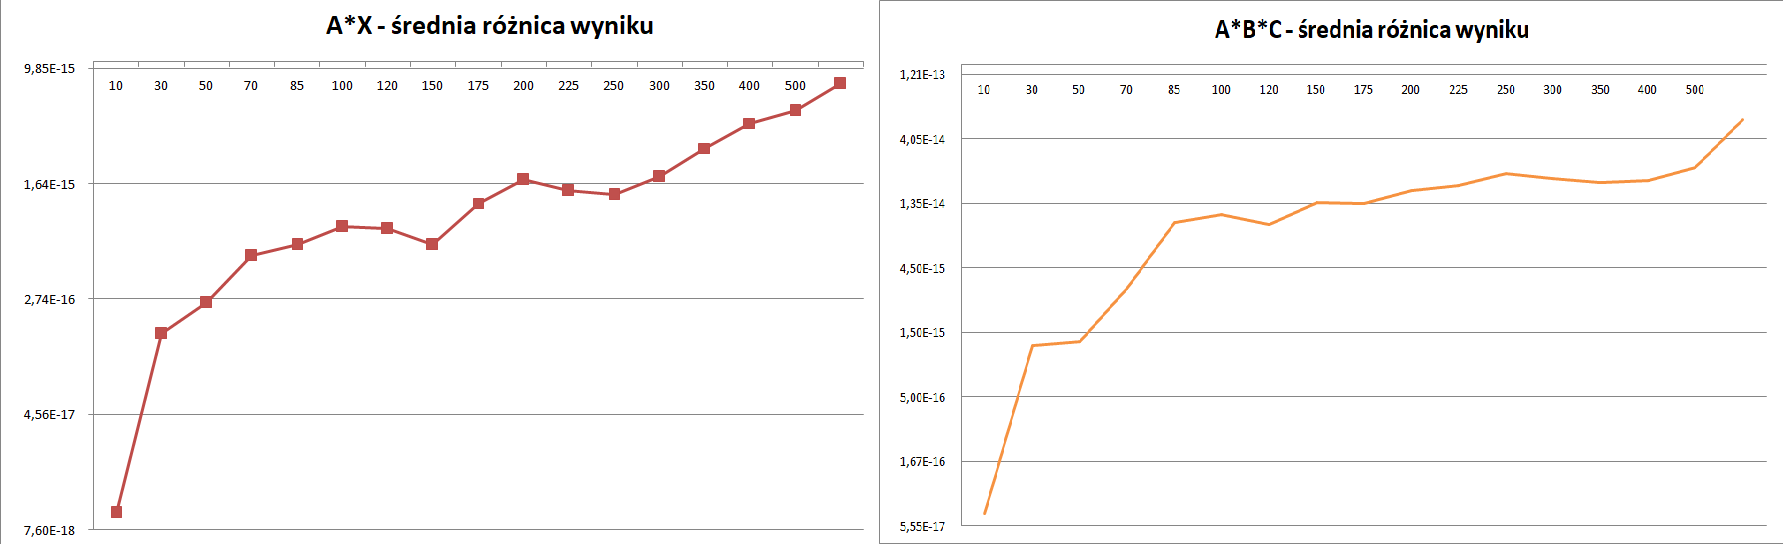
\includegraphics[width=20cm,height=7cm]{RoznicaRazem.png}}
\end{center}

Obliczenia na float wykazywały podobną tendencje, tyle że w mniejszej skali i wolniejszym tempie, więc pominę prezentacje dla tej zmiennoprzecinkowej.
W przypadku własnej precyzji, w zakresie porównania do double obliczonego przez eigen wyniki pokrywały się idealnie. Główna różnica to dłuższy czas oczekiwania na wynik.

\begin{center}
 \makebox[\textwidth]{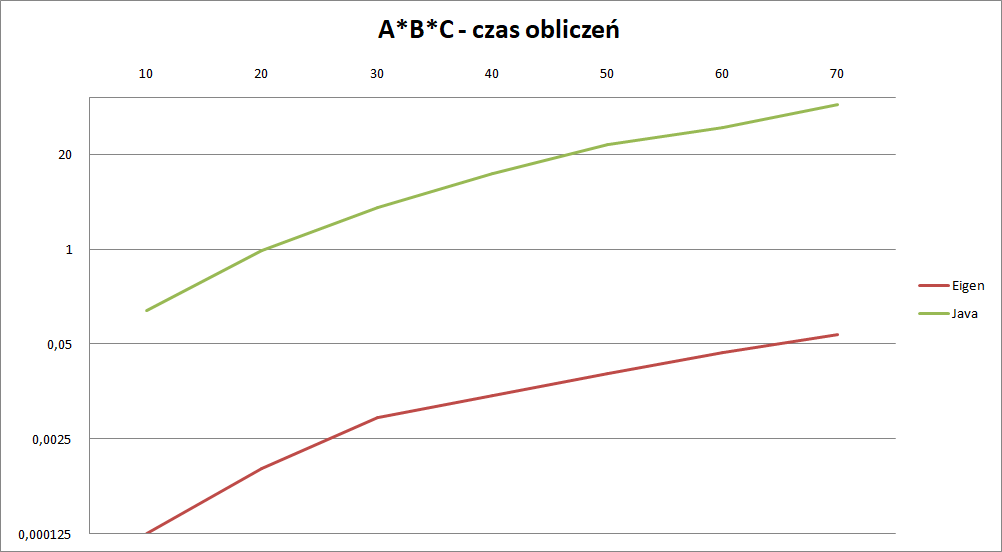
\includegraphics[width=14cm,height=7cm]{ABCCzasMy.png}}
\end{center}


\section{Rozwiązywanie układów równań liniowych}
Druga część opisuje rozwiązywanie układu równań liniowych macierzy A i wektora B.
W javie wykorzystane zostały 3 wersje metody eliminacji Gaussa:\\
\\
-bez wyboru elementu podstawowego\\
-z częściowym wyborem elementu podstawowego\\
-z pełnym wyborem elementu podstawowego\\
\\
Odnośnikiem jako poprawny wynik było podstawienie pod układ obliczonych niewiadomych.W eigen skorzystano z wyliczenia poprzez częściowy i pełny wybór.

Pierwszy wykres przedstawia różnice obliczonego układu dla wyliczonych niewiadomych i oryginalnego wektora.Tym niższa wartość w danym punkcie tym precyzyjniejszy wynik.Najlepszy okazuje się wynik wyliczony przez Eigen. Niewiele gorzej wypada Double dla pełnego wyboru elementu podstawowego.


\begin{center}
 \makebox[\textwidth]{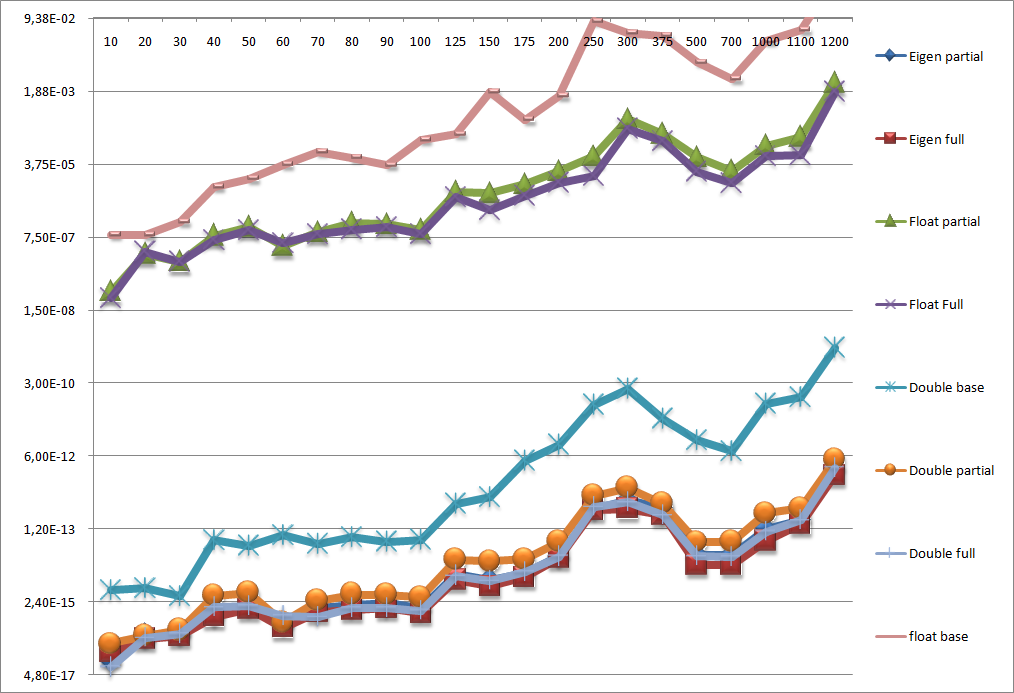
\includegraphics[width=17cm,height=10cm]{gaussPrecyzja2.png}}
\end{center}

.\\
\\
\\
\\
\\Drugi wykres przedstawia czas potrzebny do osiągnięcia rozwiązania.Chaotyczny rozkład i przenikanie przez siebie dolnych linii wynika z sytuacji, gdzie dana macierz może mieć odpowiedni układ nie wymagający jakiegokolwiek sortowania, lub ilość zamian kolumn czy wierszy jest mała. Stąd tak zbliżone wyniki.\\

\begin{center}
 \makebox[\textwidth]{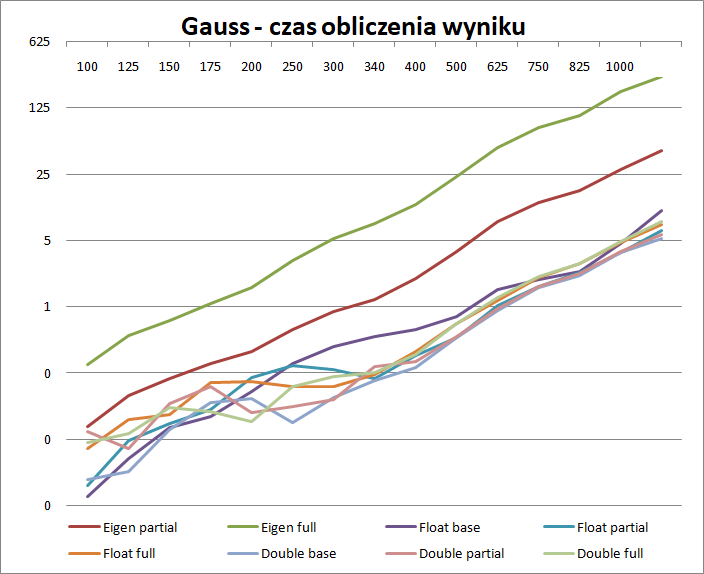
\includegraphics[width=13cm,height=10cm]{GaussCzas.png}}
\end{center}


Ostatni wykres przedstawia czas potrzebny do wyliczenia wyników dla idealnej precyzji. W istocie wynik wychodzi za każdym razem idealny. Wraz ze wzrostem macierzy, czas oczekiwania na wynik bardzo szybko rośnie co widać na dorysowanej na szaro funkcji.

\begin{center}
 \makebox[\textwidth]{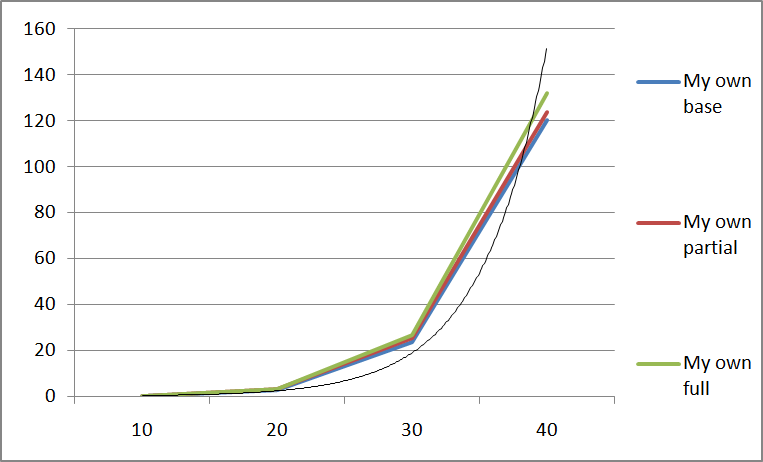
\includegraphics[width=13cm,height=7cm]{MyOwnTime.png}}
\end{center}

Obliczenia wraz ze wzrostem rozmiaru macierzy były liczone od 300 do 5 próbek. Zazwyczaj tyle wystarczało by zauważyć tendencje wzrostowe.\\
\\
\begin{tabular}{ | p{8.2cm} | p{8.2cm} | }
  \hline
  \multicolumn{2}{|c|}{Podział obowiązków} \\
  \hline
  \multicolumn{1}{|c|}{\textbf{Aleksander Kosma} }& \multicolumn{1}{|c|}{\textbf{Tomasz Adamczyk}} \\
  \hline
  -Klasa MyOwnPrecision & -Implementacja  Gaussa do Klasy MyMatrix \\\hline
  -Szkielet klasy i zapewnienie generyczności & -Klasa do generowania losowych macierzy \\\hline
  -Implementacja metod dodawania i mnożenia & -Generowanie wyniku poprzez bibliotekę Eigen w C++ \\\hline
  -Testy i generowanie wyników & -Zautomatyzowanie generowania wyników \\\hline
  -Obróbka wyników, wykresy i opracowanie & - \\\hline
  
  \hline
\end{tabular}



\end{document}